\documentclass[a4paper, 12pt]{article}

% packages
\usepackage{amssymb}
\usepackage[fleqn]{mathtools}
\usepackage{tikz}
\usepackage{enumerate}
\usepackage{bussproofs}
\usepackage{xcolor}
\usepackage[margin=1.3cm]{geometry}
\usepackage{logicproof}
\usepackage{diagbox}
\usepackage{listings}
\usepackage{graphicx}
\usepackage{lstautogobble}
\usepackage{hyperref}
\usepackage{multirow}
\usepackage{tipa}
\usepackage{pgfplots}
\usepackage{adjustbox}
\usepackage{dsfont}

% tikz libraries
\usetikzlibrary{
    decorations.pathreplacing,
    arrows,
    shapes,
    shapes.gates.logic.US,
    circuits.logic.US,
    calc,
    automata,
    positioning,
    intersections
}

\pgfplotsset{compat=1.16}

\pgfmathdeclarefunction{gauss}{2}{%
  \pgfmathparse{1/(#2*sqrt(2*pi))*exp(-((x-#1)^2)/(2*#2^2))}%
}

\allowdisplaybreaks % allow environments to break
\setlength\parindent{0pt} % no indent

% shorthand for verbatim
% this clashes with logicproof, so maybe fix this at some point?
\catcode`~=\active
\def~#1~{\texttt{#1}}

% code listing
\lstdefinestyle{main}{
    numberstyle=\tiny,
    breaklines=true,
    showspaces=false,
    showstringspaces=false,
    tabsize=2,
    numbers=left,
    basicstyle=\ttfamily,
    columns=fixed,
    fontadjust=true,
    basewidth=0.5em,
    autogobble,
    xleftmargin=3.0ex,
    mathescape=true
}
\newcommand{\dollar}{\mbox{\textdollar}} %
\lstset{style=main}

% augmented matrix
\makeatletter
\renewcommand*\env@matrix[1][*\c@MaxMatrixCols c]{%
\hskip -\arraycolsep
\let\@ifnextchar\new@ifnextchar
\array{#1}}
\makeatother

% ceiling / floor
\DeclarePairedDelimiter{\ceil}{\lceil}{\rceil}
\DeclarePairedDelimiter{\floor}{\lfloor}{\rfloor}

% custom commands
\newcommand{\indefint}[2]{\int #1 \, \mathrm{d}#2}
\newcommand{\defint}[4]{\int_{#1}^{#2} #3 \, \mathrm{d}#4}
\newcommand{\pdif}[2]{\frac{\partial #1}{\partial #2}}
\newcommand{\dif}[2]{\frac{\mathrm{d}#1}{\mathrm{d}#2}}
\newcommand{\limit}[2]{\raisebox{0.5ex}{\scalebox{0.8}{$\displaystyle{\lim_{#1 \to #2}}$}}}
\newcommand{\limitsup}[2]{\raisebox{0.5ex}{\scalebox{0.8}{$\displaystyle{\limsup_{#1 \to #2}}$}}}
\newcommand{\summation}[2]{\sum\limits_{#1}^{#2}}
\newcommand{\product}[2]{\prod\limits_{#1}^{#2}}
\newcommand{\intbracket}[3]{\left[#3\right]_{#1}^{#2}}
\newcommand{\laplace}{\mathcal{L}}
\newcommand{\fourier}{\mathcal{F}}
\newcommand{\mat}[1]{\boldsymbol{#1}}
\renewcommand{\vec}[1]{\boldsymbol{#1}}
\newcommand{\rowt}[1]{\begin{bmatrix}
    #1
\end{bmatrix}^\top}
\DeclareMathOperator*{\argmax}{argmax}
\DeclareMathOperator*{\argmin}{argmin}

\newcommand{\lto}[0]{\leadsto\ }

\newcommand{\ulsmash}[1]{\underline{\smash{#1}}}

\newcommand{\powerset}[0]{\wp}
\renewcommand{\emptyset}[0]{\varnothing}

\makeatletter
\newsavebox{\@brx}
\newcommand{\llangle}[1][]{\savebox{\@brx}{\(\m@th{#1\langle}\)}%
  \mathopen{\copy\@brx\kern-0.5\wd\@brx\usebox{\@brx}}}
\newcommand{\rrangle}[1][]{\savebox{\@brx}{\(\m@th{#1\rangle}\)}%
  \mathclose{\copy\@brx\kern-0.5\wd\@brx\usebox{\@brx}}}
\makeatother
\newcommand{\lla}{\llangle}
\newcommand{\rra}{\rrangle}
\newcommand{\la}{\langle}
\newcommand{\ra}{\rangle}
\newcommand{\crnr}[1]{\text{\textopencorner} #1 \text{\textcorner}}
\newcommand{\bnfsep}[0]{\ |\ }
\newcommand{\concsep}[0]{\ ||\ }

\newcommand{\axiom}[1]{\AxiomC{#1}}
\newcommand{\unary}[1]{\UnaryInfC{#1}}
\newcommand{\binary}[1]{\BinaryInfC{#1}}
\newcommand{\trinary}[1]{\TrinaryInfC{#1}}
\newcommand{\quaternary}[1]{\QuaternaryInfC{#1}}
\newcommand{\quinary}[1]{\QuinaryInfC{#1}}
\newcommand{\dproof}[0]{\DisplayProof}
\newcommand{\llabel}[1]{\LeftLabel{\scriptsize #1}}
\newcommand{\rlabel}[1]{\RightLabel{\scriptsize #1}}

\newcommand{\ttbs}{\char`\\}
\newcommand{\lrbt}[0]{\ \bullet\ }

% colours
\newcommand{\violet}[1]{\textcolor{violet}{#1}}
\newcommand{\blue}[1]{\textcolor{blue}{#1}}
\newcommand{\red}[1]{\textcolor{red}{#1}}
\newcommand{\teal}[1]{\textcolor{teal}{#1}}

% reasoning proofs
\usepackage{ltablex}
\usepackage{environ}
\keepXColumns
\NewEnviron{reasoning}{
    \begin{tabularx}{\textwidth}{rlX}
        \BODY
    \end{tabularx}
}
\newcommand{\proofline}[3]{$(#1)$ & $#2$ & \hfill #3 \smallskip \\}
\newcommand{\proofarbitrary}[1]{& take arbitrary $#1$ \smallskip \\}
\newcommand{\prooftext}[1]{\multicolumn{3}{l}{#1} \smallskip \\}
\newcommand{\proofmath}[3]{$#1$ & = $#2$ & \hfill #3 \smallskip \\}
\newcommand{\prooftherefore}[1]{& $\therefore #1$ \smallskip \\}
\newcommand{\proofbc}[0]{\prooftext{\textbf{Base Case}}}
\newcommand{\proofis}[0]{\prooftext{\textbf{Inductive Step}}}

% ER diagrams
\newcommand{\nattribute}[4]{
    \node[draw, state, inner sep=0cm, minimum size=0.2cm, label=#3:{#4}] (#1) at (#2) {};
}
\newcommand{\mattribute}[4]{
    \node[draw, state, accepting, inner sep=0cm, minimum size=0.2cm, label=#3:{#4}] (#1) at (#2) {};
}
\newcommand{\dattribute}[4]{
    \node[draw, state, dashed, inner sep=0cm, minimum size=0.2cm, label=#3:{#4}] (#1) at (#2) {};
}
\newcommand{\entity}[3]{
    \node[] (#1-c) at (#2) {#3};
    \node[inner sep=0cm] (#1-l) at ($(#1-c) + (-1, 0)$) {};
    \node[inner sep=0cm] (#1-r) at ($(#1-c) + (1, 0)$) {};
    \node[inner sep=0cm] (#1-u) at ($(#1-c) + (0, 0.5)$) {};
    \node[inner sep=0cm] (#1-d) at ($(#1-c) + (0, -0.5)$) {};
    \draw
    ($(#1-c) + (-1, 0.5)$) -- ($(#1-c) + (1, 0.5)$) -- ($(#1-c) + (1, -0.5)$) -- ($(#1-c) + (-1, -0.5)$) -- cycle;
}
\newcommand{\relationship}[3]{
    \node[] (#1-c) at (#2) {#3};
    \node[inner sep=0cm] (#1-l) at ($(#1-c) + (-1, 0)$) {};
    \node[inner sep=0cm] (#1-r) at ($(#1-c) + (1, 0)$) {};
    \node[inner sep=0cm] (#1-u) at ($(#1-c) + (0, 1)$) {};
    \node[inner sep=0cm] (#1-d) at ($(#1-c) + (0, -1)$) {};
    \draw
    ($(#1-c) + (-1, 0)$) -- ($(#1-c) + (0, 1)$) -- ($(#1-c) + (1, 0)$) -- ($(#1-c) + (0, -1)$) -- cycle;
}

% AVL Trees
\newcommand{\avltri}[4]{
    \draw ($(#1)$) -- ($(#1) + #4*(0.5, -1)$) -- ($(#1) + #4*(-0.5, -1)$) -- cycle;
    \node at ($(#1) + #4*(0, -1) + (0, 0.5)$) {#3};
    \node at ($(#1) + #4*(0, -1) + (0, -0.5)$) {#2};
}

% RB Trees
\tikzset{rbtr/.style={inner sep=2pt, circle, draw=black, fill=red}}
\tikzset{rbtb/.style={inner sep=2pt, circle, draw=black, fill=black}}

% Samples
\tikzset{spos/.style={inner sep=2pt, circle, draw=black, fill=blue!20}}
\tikzset{sneg/.style={inner sep=2pt, circle, draw=black, fill=red!20}}

% Joins
\newcommand\ljoin{\stackrel{\mathclap{\normalfont\mbox{\tiny L}}}{\bowtie}}
\newcommand\rjoin{\stackrel{\mathclap{\normalfont\mbox{\tiny R}}}{\bowtie}}
\newcommand\ojoin{\stackrel{\mathclap{\normalfont\mbox{\tiny O}}}{\bowtie}}

\setcounter{MaxMatrixCols}{100}

% actual document
\begin{document}
    {\sc Computing $4^\text{th}$ Year Notes} \hfill ~https://github.com/lin-e/imperial-revision~
    \rule{\textwidth}{0.1pt}
    \section*{Mathematics for Machine Learning \hfill (70015)}
        \subsection*{Lecture 1.1 - Linear Regression Intro}
            Linear regression aims to provide a solution to the supervised learning problem; we are given a dataset of $N$ examples of inputs and expected outputs, with a goal of predicting the correct output for a new input.
            Examples of this include image classification (such as digit classification) and translation.
            A curve fitting problem in 1-dimension has an input space $\in \mathbb{R}$, and an output space $\in \mathbb{R}$.
            \medskip

            To tackle this problem mathematically, we need to first describe the curve fitting problem mathematically.
            As each input is associated with a single output, this is equivalent to a function in mathematics.
            We are given a dataset of $N$ pairs, of inputs and outputs, where $\vec{x_n} \in \mathcal{X}$, which is usually $\mathbb{R}^D$ and $y_n \in \mathcal{Y}$ (usually $\mathbb{R}$ in this case); $\{(\vec{x_n}, y_n)\}_{n = 1}^N$.
            The goal is to find a function that maps from the input space to the output space \textbf{well}; $f : \mathcal{X} \to \mathcal{Y}$.
            \medskip

            We need to first find candidates for functions that can perform the predictions.
            Functions need to be parameterised, such that some numbers $\vec{\theta}$ map to a function.
            From here, we need to pick the `best' function, thus requiring us to define what good and bad functions are.
            A good function has the property $f(\vec{x_i}, \vec{\theta^*}) \approx y_i$; the output of the function closely matches the outputs of the training points.
            This can be defined with a \textbf{loss function}, for example;
            $$L(\vec{\theta}) = \summation{i = 1}{N} (y_i - f(\vec{x_i}, \vec{\theta}))^2$$
            Therefore, a good function is chosen by minimising the loss; $\vec{\theta^*} = \argmin_{\vec{\theta}}L(\vec{\theta})$.
        \subsection*{Lecture 1.2 - Scalar Differentiation}
            We can plot the loss against the parameters for a function.
            This raises two questions; how to change the parameter to make the loss smaller and how we know if we can't get a better loss.
            The derivative is defined as the limit of the difference quotient (as usual);
            $$f^\prime(x) = \dif{f}{x} = \limit{h}{0} \frac{f(x + h) - f(x)}{h}$$
            Several examples of this are as follows;
            \begin{center}
                \begin{tabular}{c|c}
                    $f(x)$ & $f^\prime(x)$ \\
                    \hline
                    $x^n$ & $nx^{n - 1}$ \\
                    $\sin(x)$ & $\cos(x)$ \\
                    $\tanh(x)$ & $1 - \tanh^2(x)$ \\
                    $e^x = \exp(x)$ & $e^x$ \\
                    $\log(x)$ & $\frac{1}{x}$
                \end{tabular}
            \end{center}
            There are also the following rules which combine the basic functions;
            \begin{itemize}
                \itemsep0em
                \item sum rule \hfill describes the derivative of sum of two functions
                    $$(f(x) + g(x))^\prime = f^\prime(x) + g^\prime(x)$$
                \item product rule \hfill similarly, for multiplication
                    $$(f(x)g(x))^\prime = f^\prime(x)g(x) + f(x)g^\prime(x)$$
                \item chain rule \hfill describes how to differentiate functions that are composed
                    $$(g \circ f)^\prime(x) = (g(f(x)))^\prime = g^\prime(f(x))f^\prime(x)$$
                \item quotient rule \hfill describes division, special case of the product rule
                    $$\left(\frac{f(x)}{g(x)}\right)^\prime = \frac{f^\prime(x)g(x) - f(x)g^\prime(x)}{(g(x))^2}$$
            \end{itemize}
            This tells us how to change the input in the function; the gradient tells us how much the output changes based on an increase in the input.
            We first compute the derivative function at a point to find the point's gradient.
            If the gradient is negative, this tells us the function will decrease if we increase the input (hence increase to minimise), and vice versa; decrease for positive gradients - this is the idea behind gradient descent.
            \medskip

            Similarly, we know we are done (at a minimum for the loss function) when there is nothing that can be done to lower the output, hence the gradient must be 0.
            However, this isn't sufficient to tell us that we have reached a minimum, as a maximum also has a gradient of zero.
            A minimum has a decreasing function followed by an increasing function; hence the gradient of the gradient (second derivative) is positive.
            \medskip

            However, this only gives us a local minima.
            We should be concerned with getting stuck in a local minima (rather than a global minima) when dealing with non-convex functions.
            Working through a simple example, with a linear regression problem (aiming to find an optimal $a$) - the final step takes the second derivative to verify we have a minimum;
            \begin{align*}
                f(x) & = a \cdot x \\
                L(a) & = \summation{n = 1}{N} (f(x_n) - y_n)^2 \\
                \dif{L}{a} & = \summation{n = 1}{N} 2(ax_n - y_n)x_n \\
                & = \summation{n = 1}{N} 2ax_n^2 - 2x_ny_n \\
                & = 0 \\
                2a\summation{n}{} x_n^2 & = \summation{n}{} 2x_ny_n \\
                a & = \frac{\summation{n}{} 2x_ny_n}{\summation{n}{} x_n^2} \\
                \dif{^2L}{a^2} & = \summation{n = 1}{N} 2x_n^2 \\
                & \geq 0
            \end{align*}
        \subsubsection*{Lecture 1.3 - Scalar-by-vector Differentiation}
            The previous example is too simple for real applications - we will need to differentiate by more parameters (vectors).
            Consider the following example, a polynomial, which has 4 vectors parametising it - each vector now corresponds to a single cubic polynomial;
            \begin{align*}
                f(x) & = \theta_3x^3 + \theta_2x^2 + \theta_1x + \theta_0 \\
                & = \vec{\theta}^\top\vec{\phi}(x) \\
                \vec{\phi}(x) & = \begin{bmatrix}
                    x^3 & x^2 & x & 1
                \end{bmatrix}^\top
            \end{align*}
            Our goal still remains to understand how a function changes with our parameter and to characterise what an optimum is for a function of a vector.
            Both of these change a multi-dimensional problem into many 1-dimensional problems.
            \medskip

            We want to change it into a 1-dimensional question; instead of asking about a change to $\vec{\theta}$, we ask what happens when we move along a particular line / direction.
            A directional derivative is how much the function changes, when we move in a direction $\vec{v}$;
            $$\nabla_{\vec{v}}L(\vec{\theta}) = \limit{h}{0}\frac{L(\vec{\theta} + h\vec{v}) - L(\vec{\theta})}{h}$$ % assuming a mistake in the slides, the -L(theta) wasn't there
            The distance that we move away from the starting point ($\vec{\theta}$) is determined by \textbf{both} the norm / scale of the direction vector $\vec{v}$, as well as $h$.
            If we can understand how the function changes based on a change in \textbf{any} direction, we can fully characterise differentiation with respect to a vector.
            \medskip

            Consider the following example, where we deal with two parameters (also notice the second equality holds as the values in \violet{violet} are equal and cancel each other out);
            \begin{align*}
                \nabla_{\vec{v}}L(\vec{\theta}) & = \limit{h}{0}\frac{L(\theta_1 + hv_1, \theta_2 + hv_2) - L(\theta_1, \theta_2)}{h} \\
                & = \limit{h}{0}\underbrace{\frac{L(\theta_1 + hv_1, \theta_2 + hv_2) - \violet{L(\theta_1, \theta_2 + hv_2)}}{h}}_\text{only change in first parameter} + \underbrace{\frac{\violet{L(\theta_1, \theta_2 + hv_2)} - L(\theta_1, \theta_2)}{h}}_\text{only change in second parameter} \\
                & = \limit{h}{0}\frac{L(\theta_1 + h^\prime, \theta_2 + h^\prime\frac{v_2}{v_1}) - \violet{L(\theta_1, \theta_2 + h^\prime\frac{v_2}{v_1})}}{\frac{h^\prime}{v_1}} + \frac{\violet{L(\theta_1, \theta_2 + h^{\prime\prime})} - L(\theta_1, \theta_2)}{\frac{h^{\prime\prime}}{v_2}} \\
                & = \pdif{L}{\theta_1}v_1 + \pdif{L}{\theta_2}v_2
            \end{align*}
            This means that we can find the gradient in any direction with the partial derivatives, as we chose arbitrary $v_1, v_2$.
            With a partial derivative, we change only one coordinate at a time - see the following for a function $f : \mathbb{R}^N \to \mathbb{R}$;
            \begin{align*}
                y & = f(\vec{x}) \\
                x & = \begin{bmatrix}
                    x_1 \\ \vdots \\ x_N
                \end{bmatrix} \\
                \pdif{f}{x_i} & = \limit{h}{0} \frac{f(x_1, \dots, x_{i - 1}, \violet{x_i + h}, x_{i + 1}, \dots, x_N) - f(\vec{x})}{h}
            \end{align*}
            The Jacobian vector collects all partial derivatives into a row vector;
            $$\dif{f}{\vec{x}} = \begin{bmatrix}
                \pdif{f}{x_1} & \cdots & \pdif{f}{x_N}
            \end{bmatrix} \in \mathbb{R}^{1 \times N}$$
            We now want to know which direction to go in, to decrease the value of the function the most.
            The directional derivative can be written as the inner product;
            $$\nabla_{\vec{v}}f(\vec{\theta}) = \dif{f}{\vec{\theta}}\vec{v} = \left|\dif{f}{\vec{\theta}}\right|\left|\vec{v}\right| \cos \beta$$
            We can maximise this by making $\cos \beta$ as large as possible, since the norms of the two vectors are fixed.
            If we choose a unit vector $\vec{v}$, we want the largest value possible, hence $\cos \beta = 1$, so the angle between the vectors should be zero (such that $\beta = 0$).
            As such, we move in the direction of the Jacobian / gradient vector.
            \medskip

            We can reuse the intuition from the 1-D case, where moving in either direction doesn't change your value - the directional derivative should be zero in \textbf{all directions} (hence the zero vector, $\vec{0}$).
            Additionally, to verify it's a minimum, we want the second directional derivative to also be positive in \textbf{all directions}.
        \subsection*{Lecture 1.4 - Vector-by-vector Differentiation}
            Recall the motivating example of linear regression;
            $$L(\vec{\theta}) = \summation{n = 1}{N}(y_n - \vec{\phi}(x_n)^T\vec{\theta})^2 = || \vec{y} - \violet{\mat{\Phi}(X) \vec{\theta}} ||^2$$
            We could either manually take partial derivatives of $L$, which would be laborious, or consider it as a composition of a vector-to-vector function (the \violet{matrix multiplication}) and a vector-to-scalar function (the norm of the vector squared);
            \begin{center}
                \hfill $f(\vec{g}(\vec{\theta}))$ \hfill $f : \mathbb{R}^D \to \mathbb{R}$ \hfill $g : \mathbb{R}^E \to \mathbb{R}^D$ \hfill
            \end{center}
            There is a multivariate chain rule, for scalars it is as follows (where $f$ is a function of $a$ and $b$, both of which are functions of $t$);
            $$\dif{f(a(t), b(t))}{t} = \pdif{f}{a} \dif{a}{t} + \pdif{f}{b} \dif{b}{t}$$
            This can be generalised as follows, for $\vec{g}(t) \in \mathbb{R}^D$, and both are vectors - allowing us to write it as an inner product;
            $$\dif{f(\vec{g}(t))}{t} = \summation{i = 1}{D} \pdif{f}{g_i} \dif{g_i}{t} = \underbrace{\dif{f}{\vec{g}}}_\text{row} \cdot \underbrace{\dif{\vec{g}}{t}}_\text{col}$$
            This only works as we've defined the differentiation of a function with respect to a vector as a row vector - which we will use for the remainder of the course.
            Similarly, the second part of the sum is the derivative of a column vector, which remains a column vector.
            Consider the following example, with $f : \mathbb{R}^2 \to \mathbb{R}$ and $\vec{x} : \mathbb{R} \to \mathbb{R}^2$;
            \begin{align*}
                f(\vec{x}) & = f(x_1, x_2) \\
                & = x_1^2 + 2x_2 \\
                \vec{x}(t) & = \begin{bmatrix}
                    x_1(t) \\ x_2(t)
                \end{bmatrix} \\
                & = \begin{bmatrix}
                    \sin(t) \\ \cos(t)
                \end{bmatrix} \\
                \dif{f}{\vec{x}} & \in \mathbb{R}^{1 \times 2} \\
                \dif{\vec{x}}{t} & \in \mathbb{R}^2 \\
                \dif{f}{t} & = \violet{\dif{f}{\vec{x}}} \teal{\dif{\vec{x}}{t}} \\
                & = \violet{\begin{bmatrix}
                    \pdif{f}{x_1} & \pdif{f}{x_2}
                \end{bmatrix}} \teal{\begin{bmatrix}
                    \pdif{x_1}{t} \\ \pdif{x_2}{t}
                \end{bmatrix}} \\
                & = \violet{\begin{bmatrix}
                    2\sin(t) & 2
                \end{bmatrix}} \teal{\begin{bmatrix}
                    \cos(t) \\ -\sin(t)
                \end{bmatrix}} \\
                & = 2\sin(t)(\cos(t) - 1)
            \end{align*}
            A similar rule applies when differentiating with respect to a vector (note previously we only did it with respect to a scalar).
            Similarly, this just requires collecting all the partial derivatives, and the same chain rule applies for $\vec{g}(\vec{x}) \in \mathbb{R}^D$;
            $$\pdif{f(\vec{g}(\vec{x}))}{x_j} = \summation{i = 1}{D} \pdif{f}{g_i} \dif{g_i}{x_j}$$ % assuming slides incorrect again, it uses f(g(t)) instead of f(g(x))
            Once collected, this becomes matrix multiplication, which can be written in vector form;
            $$\dif{f(\vec{g}(\vec{x}))}{\vec{x}} = \underbrace{\dif{f}{\vec{g}}}_\text{row} \cdot \underbrace{\dif{\vec{g}}{\vec{x}}}_\text{mat}$$
            Note that the matrix is the derivative of a column vector ($\vec{g}$) with respect to an input vector $\vec{x}$.
            We instead put the elements in each row (similar to how we did it for a vector by scalar) - the elements of $\vec{g}$ ($i$) are along the column, and the dimensions of the derivative ($j$) are along the row.
            If $f$ gave a vector as an output, we'd end up with a matrix by matrix multiplication.
            \medskip

            Consider the following example, where we have $f : \mathbb{R}^N \to \mathbb{R}^M$, $\vec{y} = \vec{f}(\vec{x}) \in \mathbb{R}^M$, and $\vec{x} \in \mathbb{R}^N$;
            $$\begin{bmatrix}
                \violet{y_1} \\ \vdots \\ \teal{y_M}
            \end{bmatrix} = \begin{bmatrix}
                \violet{f_1(\vec{x})} \\ \vdots \\ \teal{f_M(\vec{x})}
            \end{bmatrix} = \begin{bmatrix}
                \violet{f_1(x_1, \dots, x_N)} \\ \vdots \\ \teal{f_M(x_1, \dots, x_N)}
            \end{bmatrix}$$
            The collection of all partial derivatives is called a Jacobian matrix;
            $$\begin{bmatrix}
                \violet{\dif{y_1}{\vec{x}}} \\ \vdots \\ \teal{\dif{y_M}{\vec{x}}}
            \end{bmatrix} = \begin{bmatrix}
                \violet{\pdif{f_1}{x_1}} & \violet{\cdots} & \violet{\pdif{f_1}{x_N}} \\
                \vdots & & \vdots \\
                \teal{\pdif{f_M}{x_1}} & \teal{\cdots} & \teal{\pdif{f_M}{x_N}}
            \end{bmatrix} \in \mathbb{R}^{M \times N}$$
            In general, a function $\vec{f} : \mathbb{R}^N \to \mathbb{R}^M$ has a gradient that is a matrix $\mathbb{R}^{M \times N}$, or has the number of target dimensions ($M$) $\times$ the number of input dimensions ($N$);
            $$\mathrm{d}\vec{f}[m, n] = \pdif{f_m}{x_n}$$
            Recall that for matrix multiplication, the second dimension of the first matrix must match with the first dimension of the second matrix.
            A function composition is constrained that the output dimension of $\vec{h}$ must be the same as the input dimension of $\vec{g}$ to compute $\vec{g}(\vec{h}(\vec{x}))$ when we have $\vec{f}(\vec{x}) = (\vec{g} \circ \vec{h})(\vec{x})$.
            This ensures the shapes of the chain rule will \textbf{always} work out.
            For $\vec{f}: \mathbb{R}^N \to \mathbb{R}^M$, $\vec{g}: \mathbb{R}^L \to \mathbb{R}^M$, and $\vec{h}: \mathbb{R}^N \to \mathbb{R}^L$, we have the following shapes;
            $$\underbrace{\dif{\vec{f}}{\vec{x}}}_{M \times N} = \underbrace{\dif{\vec{g}}{\vec{h}}}_{M \times L} \underbrace{\dif{\vec{h}}{\vec{x}}}_{L \times N}$$
            Consider the following example, of a matrix multiplication $\vec{f}(\vec{x}) = \mat{A}\vec{x}$ where we have $\mat{A} \in \mathbb{R}^{M \times N}$ and $\vec{x} \in \mathbb{R}^N$;
            \begin{align}
                \begin{bmatrix}
                    y_1 \\ \vdots \\ y_M
                \end{bmatrix} & = \begin{bmatrix}
                    f_1(\vec{x}) \\ \vdots \\ f_M(\vec{x})
                \end{bmatrix} \\
                & = \begin{bmatrix}
                    A_{1, 1}x_1 + A_{1, 2}x_2 + \cdots + A_{1, N}x_N \\
                    \vdots \\
                    A_{M, 1}x_1 + A_{M, 2}x_2 + \cdots + A_{M, N}x_N
                \end{bmatrix} \\
                f_i(\vec{x}) & = \summation{k = 1}{N} A_{i, k}x_k \\
                \pdif{f_i}{x_j} & = \summation{k}{} A_{i, k} \pdif{x_k}{x_j} \\
                & = \summation{k}{} A_{i, k} \delta_{k, j} \\
                & = A_{i, j}
            \end{align}
            Note the following steps in particular;
            \begin{enumerate}[(1)]
                \itemsep0em
                \setcounter{enumi}{2}
                \item write out each scalar in the vector with index notation by writing the sum explicitly allowing us to take the derivative of an arbitrary element in the output vector with respect to an arbitrary element in the input vector
                \item take differential operator inside by sum rule
                \item matrix value is constant, so we end up taking a partial derivative of $x_k$ by $x_j$ - partial derivative only changes $x_j$ and keeps everything else constant, hence it will be zero when $k \neq j$ and 1 when $k = j$ (indicator function, $\delta$)
                \item end up with $A_{i, j}$ as it's the only case the indicator function is non-zero
            \end{enumerate}
            Therefore, we get the result that $\dif{f}{x} = \mat{A} \in \mathbb{R}^{M \times N}$.
            \medskip

            Consider the following, which is similar to the loss function, where $\vec{x} \in \mathbb{R}^N, \mat{A} \in \mathbb{R}^{M \times N}, \vec{e}, \vec{y} \in \mathbb{R}^M$;
            \begin{align*}
                L(\vec{e}) & = \frac{1}{2} || \vec{e} ||^2 \\
                & = \frac{1}{2} \vec{e}^\top\vec{e} \\
                \vec{e} & = \vec{y} - \mat{A}\vec{x} \\
                \dif{L}{\vec{x}} & = \pdif{L}{\vec{e}} \pdif{\vec{e}}{\vec{x}} \\
                \pdif{L}{e_i} & = \pdif{}{e_i} \summation{j}{} \frac{1}{2} e_j^2 \\
                & = \summation{j}{} \frac{1}{2} 2e_j \pdif{e_j}{e_i} \\
                & = e_i \\
                \pdif{L}{\vec{e}} & = \vec{e}^\top \\
                \pdif{\vec{e}}{\vec{x}} & = -\mat{A} \\
                \pdif{L}{\vec{x}} & = e^\top(-\mat{A}) \\
                & = -(\vec{y} - \mat{A}\vec{x})^\top\mat{A}
            \end{align*}
        \subsection*{Lecture 1.5 - Hessians}
            We still want to get the second derivative, in order to verify that we have a minima and not a maxima.
            The chain rule we have in place only works with derivatives of scalars, or column vectors (when differentiating with respect to vectors).
            We've currently defined the vertical axis to be outputs and the horizontal axis for variables we're differentiating by.
            This convention no longer holds when we are taking second derivatives, we we need to take the second derivative along a row vector;
            $$\nabla_{\vec{v}}\underbrace{\left[\dif{f}{\vec{\theta}}\vec{v}\right]}_\text{scalar} = \underbrace{\dif{}{\vec{\theta}}\left[\dif{f}{\vec{\theta}}\vec{v}\right]}_\text{row vector}\vec{v}$$
            Solving this in a way that only involves taking derivatives with respect to scalars;
            \setcounter{equation}{0}
            \begin{align}
                \dif{f}{\vec{\theta}}\vec{v} & = \summation{j}{} \pdif{f}{\theta_j}v_j \\
                \pdif{}{\theta_i}\left[\dif{f}{\vec{\theta}}\vec{v}\right] & = \summation{j}{} \pdif{}{\theta_j}\pdif{f}{\theta_j}v_j \\
                & = \summation{j}{} \pdif{^2f}{\theta_i\partial \theta_j} v_j \\
                \nabla_{\vec{v}}\left[\dif{f}{\vec{\theta}}\vec{v}\right] & = \vec{v}^\top\mat{H}\vec{v}
            \end{align}
            This involves the following steps;
            \begin{enumerate}[1.]
                \itemsep0em
                \item expand out in terms of summation components (partial derivatives multiplied by vector component)
                \item take partial derivative of the scalar, using sum rule
                \item obtain a row vector where we multiply against the second partial derivatives
                \item the matrix $\mat{H}$ (Hessian) contains all second partial derivatives of the function $f$
            \end{enumerate}
            We are at the minimum if $\mat{H}$ is positive definite ($\forall \vec{v}\ \vec{v}^\top\mat{H}\vec{v} \geq 0$) - positive eigenvalues.
        \subsection*{Lecture 2 - Matrix Derivatives and Backpropagation}
            Defining a function with respect to a number of parameters, and taking a derivative (by doing many simple problems) can be time consuming.
            % $$\pdif{L}{\vec{\theta}} = \pdif{}$$

            Consider a loss function;
            \begin{align*}
                L & = \frac{1}{2} || \vec{e} ||^2 & \vec{e} \in \mathbb{R}^N \\
                \vec{e} & = \vec{y} - \mat{A}\vec{c} & \mat{A} \in \mathbb{R}^{N \times D} \\
                \vec{c} & = \sin \vec{x} & \vec{x} \in \mathbb{R}^D \\
                % \dif{L}{\vec{x}} & 
                \pdif{L}{x_j} & = \pdif{}{x_j} \frac{1}{2} \summation{n = 1}{N} \left(y_n - \summation{i}{} A_{n, i} \sin x_i\right)^2 \\
                & = \frac{1}{2} \cdot 2 \cdot \summation{n = 1}{N} \left(y_n - \summation{i}{} A_{n, i} \sin x_i\right) \cdot \pdif{}{x_j} \left[y_n - \summation{i}{} A_{n, i} \sin x_i\right] \\
                & = \summation{n = 1}{N} \left(y_n - \summation{i}{} A_{n, i} \sin x_i\right) \summation{i}{} \pdif{}{x_j} (A_{n, i} \sin x_i) \\
                & = \summation{n = 1}{N} \left(y_n - \summation{i}{} A_{n, i} \sin x_i\right) \cdot -\summation{i}{} A_{n, i} \cos x_i \pdif{x_i}{x_j} \\
                & = \summation{n = 1}{N} \left(y_n - \summation{i}{} A_{n, i} \sin x_i\right) \cdot -\summation{i}{} A_{n, i} \cos x_i \delta_{ij} \\
                & = \summation{n = 1}{N} \left(y_n - \summation{i}{} A_{n, i} \sin x_i\right) \cdot - A_{n, j} \cos x_j \\
                \dif{L}{\vec{x}} & = \underbrace{\dif{L}{\vec{e}}}_{1 \times N} \cdot \underbrace{\dif{\vec{e}}{\vec{c}}}_{N \times D} \cdot \underbrace{\dif{\vec{c}}{\vec{x}}}_{D \times D} \\
                \pdif{L}{e_j} & = \pdif{}{e_j} \left[\frac{1}{2} \summation{n = 1}{N} e_n^2 \right] \\
                & = \frac{1}{2} \summation{n = 1}{N} \pdif{}{e_j} e_n^2 \\
                & = \summation{n}{} e_n \delta_{nj} \\
                & = e_j \\
                \pdif{e_i}{c_j} & = \pdif{}{c_j} \left[y_i - \summation{k}{} A_{i, k}c_k\right] \\
                & = -\summation{k}{} A_{i,k} \pdif{c_k}{c_j} \\
                & = -\summation{k}{} A_{i,k} \delta_{kj} \\
                & = -A_{i,j} \\
                \intertext{collect $j$s along row and $i$s down column}
                \dif{\vec{e}}{\vec{c}} & = -\mat{A} \\
                \pdif{c_i}{x_j} & = \pdif{}{x_j} \sin x_i \\
                & = \cos x_i \pdif{x_i}{x_j} \\
                & = (\cos x_i) \delta{ij} & \text{note}
            \end{align*}
            Note that previously we only had sums with the indicator function; in this case, we only have $\cos x_i$ along the diagonal, and zeroes elsewhere.
            \medskip

            Consider the linear regression problem;
            \begin{align*}
                L(\vec{\theta}) & = \frac{1}{2} || \vec{y} - \mat{\Phi}(\vec{X}) \vec{\theta} ||^2 \\
                \vec{\theta} & \in \mathbb{R}^3 \\
                \mat{\Phi}(\vec{X}) & \in \mathbb{R}^{N \times 3} \\
                \vec{y} & \in \mathbb{R}^N \\
                \vec{\phi}(x) & = \begin{bmatrix}
                    1 \\ x \\ x^2
                \end{bmatrix} \\
                \mat{\Phi}(\vec{X}) & = \begin{bmatrix}
                    \vec{\phi}^\top(x_1) \\
                    \vec{\phi}^\top(x_2) \\
                    \vdots
                \end{bmatrix} \\
                f(x) & = \vec{\phi}(x)^\top\vec{\theta} \\
                & = \theta_0 + \theta_1x + \theta_2x^2 \\
                L(\vec{e}) & = \frac{1}{2} || \vec{e} ||^2 \\
                \vec{e} & = \vec{y} - \mat{\Phi}(\vec{X})\vec{\theta} \\
                \dif{L}{\vec{\theta}} & = \dif{L}{\vec{e}} \cdot \dif{\vec{e}}{\vec{\theta}} \\
                \dif{L}{\vec{e}} & = \vec{e}^\top \\
                \dif{\vec{e}}{\vec{\theta}} & = -\mat{\Phi}(\vec{X}) \\
                & = (\vec{y} - \mat{\Phi}(\vec{X})\vec{\theta})^\top \cdot - \mat{\Phi}(\vec{X}) \\
                & = 0 \\
                \vec{\theta}^\top \mat{\Phi}(\vec{X})^\top\mat{\Phi}(\vec{X}) & = \vec{y}^\top\mat{\Phi}(\vec{X}) \\
                \vec{\theta}^\top \underbrace{[\mat{\Phi}(\vec{X})^\top\mat{\Phi}(\vec{X})][\mat{\Phi}(\vec{X})^\top\mat{\Phi}(\vec{X})]^{-1}}_{\mat{I}} & = \vec{y}^\top\mat{\Phi}(\vec{X})[\mat{\Phi}(\vec{X})^\top\mat{\Phi}(\vec{X})]^{-1}
            \end{align*}
            The basis function can also be a learnable feature, with $\phi : \mathbb{R}^D \to \mathbb{R}^L$ and $\sigma$ being an activation function;
            \begin{align*}
                \vec{x} \in \mathbb{R}^D \\
                \vec{\theta} \in \mathbb{R}^L \\
                f(\vec{x}) & = \vec{\phi}(\vec{x})^\top \vec{\theta} \\
                \vec{\phi}(x) & = \sigma(\mat{A}\vec{x} + \vec{b})
            \end{align*}
            This can be repeated deeper by replacing the $\vec{x}$ with $\vec{\phi^\prime}(\vec{x})$ (with $\mat{A^\prime}$ and $\vec{b^\prime}$ similarly), and so on.
            The idea is that we have a layer that takes in the output of the previous layer as follows (eventually, this stops with $f_0$ being $x$, the input);
            $$f_l (f_{l - 1}) = \sigma(\mat{A_l} f_{l - 1} + \vec{b_l})$$
            Note for brevity, we combine $\mat{A_i}$ and $\vec{b_i}$ as $\theta_i$;
            \begin{center}
                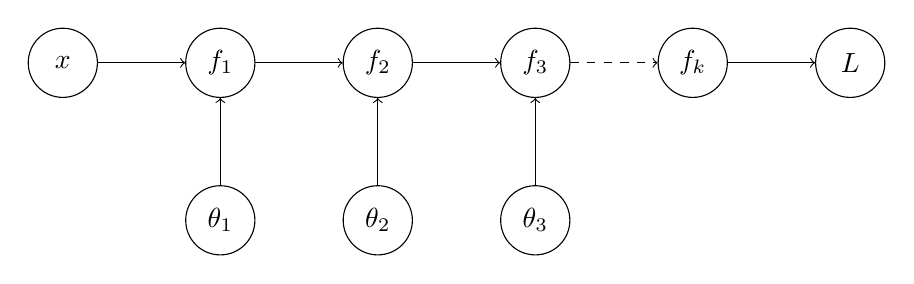
\begin{tikzpicture}[x=2cm, y=2cm]
                    \node[state] (x) at (0, 0) {$x$};
                    \node[state] (f1) at (1, 0) {$f_1$};
                    \node[state] (f2) at (2, 0) {$f_2$};
                    \node[state] (f3) at (3, 0) {$f_3$};
                    \node[state] (fk) at (4, 0) {$f_k$};
                    \node[state] (l) at (5, 0) {$L$};
                    \node[state] (t1) at (1, -1) {$\theta_1$};
                    \node[state] (t2) at (2, -1) {$\theta_2$};
                    \node[state] (t3) at (3, -1) {$\theta_3$};

                    \draw
                    (x) edge[->] (f1)
                    (f1) edge[->] (f2)
                    (f2) edge[->] (f3)
                    (f3) edge[->, dashed] (fk)
                    (fk) edge[->] (l)
                    (t1) edge[->] (f1)
                    (t2) edge[->] (f2)
                    (t3) edge[->] (f3);
                \end{tikzpicture}
            \end{center}
            If we want to learn in this model, we need to take derivatives with respect to all parameters we've defined ($\mat{A}$ and $\vec{b}$ in each layer).
            However, the former is a matrix; hence we need to take the derivative of a function with respect to a matrix, such as (note that this is no longer matrix multiplication, even if they both look like matrices; will be explained later);
            $$\dif{}{\theta} \vec{x}^\top \mat{A}(\theta) \vec{x} \text{ or } \dif{}{\mat{A}} || \mat{A}\vec{x} - \vec{y} ||^2$$
            When taking the derivative of a vector with respect to a vector, we had two indices which could be nicely represented in a matrix.
            But in the case of differentiating with respect to a matrix, we have the indices of the vector, as well as a grid of indices in the matrix.
            \medskip

            Functions of matrices are no different to functions of vectors; they're still just functions of many different numbers - hence a function of a matrix $\mat{A} \in \mathbb{R}^{M \times N}$ remains a multivariate function.
            \begin{align*}
                f(\mat{A}) & = || \mat{A}\vec{x} - \vec{y} ||^2 \\
                f(A_{1, 1}, A_{2, 1}, \dots, A_{M, 1}, \dots, A_{M, N}) & = \summation{i}{} \left(\summation{i,j}{} A_{i, j} x_j - y_i\right)
            \end{align*}
            The chain rule remains the same; where we compute all the partial derivatives with respect to the elements;
            \begin{align*}
                f(\vec{g}) = || \vec{g} ||^2 \\
                \vec{g}(\mat{A}) & = \mat{A}\vec{x} - \vec{y} \\
                \pdif{f}{A_{i, j}} & = \summation{k}{} \pdif{f}{g_k} \pdif{g_k}{A_{i, j}}
            \end{align*}
            Another example;
            \begin{align*}
                f(\mat{A}) & = \vec{x}^\top\mat{A}\vec{x} \\
                \pdif{f}{\theta} & = \summation{j,k}{} \pdif{f}{A_{j, k}} \pdif{A_{j, k}}{\theta}
            \end{align*}
            The difficulty lies in defining the notation that uses well-defined mathematical operations.
            The chain rule worked well before as we had a nice multiplication in the form of matrix multiplication; this is no longer the case here (see the note prior).
            Recall the previous notation;
            $$\dif{f}{\theta} = \dif{f}{\mat{A}} \dif{\mat{A}}{\theta} \text{ and } \dif{f}{\mat{A}} = \dif{f}{\vec{g}} \dif{\vec{g}}{\mat{A}}$$
            A derivative of a vector with respect to a matrix is a rank 3 tensor (a vector can be seen as a rank 1 tensor, and a matrix as rank 2).
            This representation with higher-dimensional tensors generalises well.
            Recall that a function $\vec{f} : \mathbb{R}^N \to \mathbb{R}^M$ ($M$ target dimensions and $N$ input dimensions) has the following;
            $$\dif{\vec{f}}{\vec{x}} \in \mathbb{R}^{M \times N}\text{,\ \ \ \ } \mathrm{d}\vec{f}[m, n] = \pdif{f_m}{x_n}$$
            This generalises when the sizes of the inputs are matrices instead, for example $\mat{f} : \mathbb{R}^{M \times N} \to \mathbb{R}^{P \times Q}$, where the gradient is a tensor;
            $$\dif{\mat{f}}{\mat{X}} \in \mathbb{R}^{M \times N}\text{,\ \ \ \ } \mathrm{d}\mat{f}[p, q, m, n] = \pdif{f_{p, q}}{X_{m, n}}$$
            Applying the chain rule to a particular matrix valued function - take the example of $f \in \mathbb{R}$ being a scalar function of $\mat{A} \in \mathbb{R}^{(P \times Q) \times (N \times M)}$, which is a function of $\vec{\theta} \in \mathbb{R}^L$;
            \setcounter{equation}{0}
            \begin{align}
                \underbrace{\dif{f}{\vec{\theta}}}_{1 \times L} & = \underbrace{\dif{f}{\mat{A}}}_{1 \times (N \times M)} \underbrace{\dif{\mat{A}}{\vec{\theta}}}_{(N \times M) \times L} \\
                & = \dif{f}{\mathrm{vec}\vec{A}} \cdot \dif{\mathrm{vec}\vec{A}}{\vec{\theta}} \\
                \mathrm{vec}\begin{bmatrix}
                    a & b \\
                    c & d
                \end{bmatrix} & = \begin{bmatrix}
                    a \\ c \\ b \\ d
                \end{bmatrix}
            \end{align}
            \begin{enumerate}[(1)]
                \itemsep0em
                \item the issue is that we end up with a tensor $\mathbb{R}^{(N \times M) \times L}$
                \item we're now back to doing differentiating with vectors, leading to matrix multiplication
                \item note that changing a matrix into a vector gives a column vector of the matrix by columns
            \end{enumerate}
            Automatic differentiation packages keep track of all these axes in these higher order tensors which contain these derivatives and figure out which axes to sum over by looking at the input shape of the function $f : \mathbb{R}^{N \times M} \to \mathbb{R}$, consistent with the matrix valued chain rule.
            The most unambiguous way to deal with this is to write it all as a vector, leading to matrix multiplication.
\end{document}